\section{Final Velocity Model}
The expression for the output torque, \si{\tau_m}, of the motor model, \eqref{eq:Totaltorquewithcurrentexpression}, along with the transfer function for the mechanical part, \eqref{eq:mechanicalTransFerfunction}, delivers the information needed to make a visual representation of the velocity model. The input is the supply voltage, \si{U_a(s)} delivered to the motor and the output is the vehicles velocity, \si{V(s)}, see \figref{fig:BlockDiagramDrivetrainComplicated}. 
%
\begin{figure}[H]
	\centering
	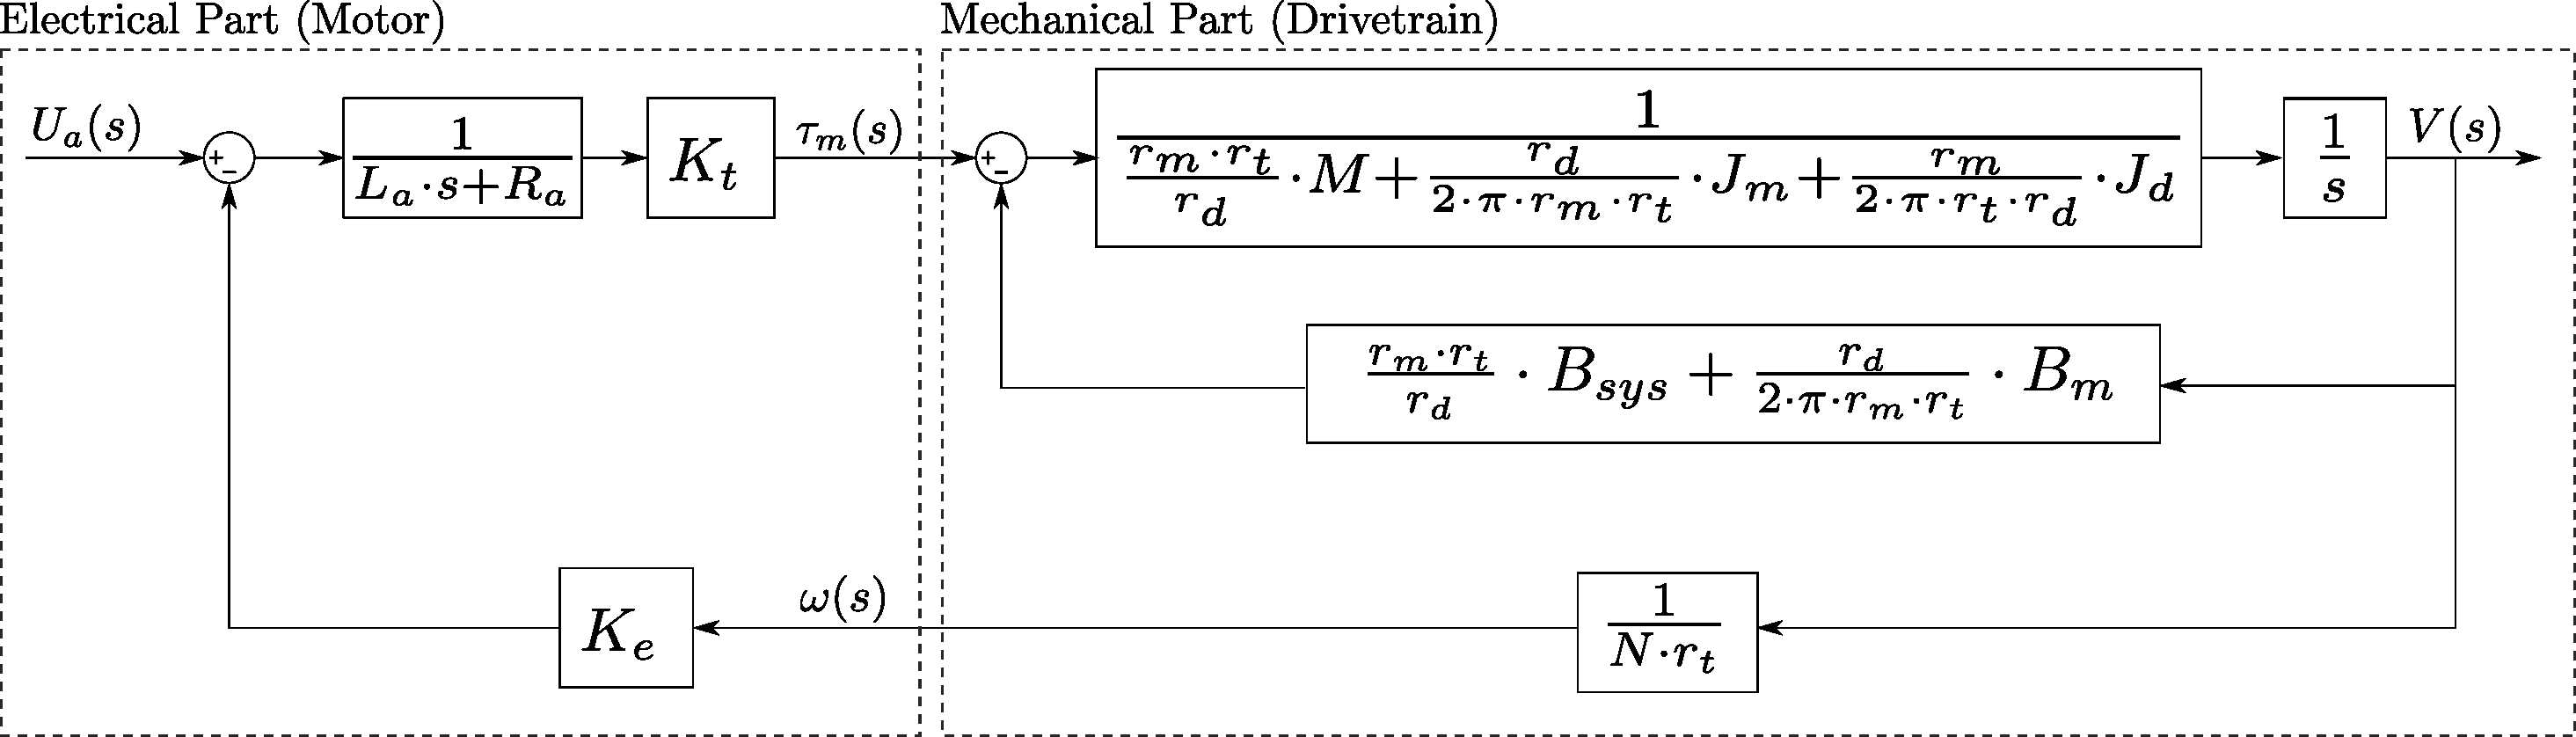
\includegraphics[width=\textwidth]{figures/totalVelocityModelDiagramComplicated.pdf}
	\caption{A block diagram of the combined drivetrain}
	\label{fig:BlockDiagramDrivetrainComplicated}
\end{figure}
%
Inspecting the above model of the drivetrain, the following two terms are extracted for closer analysis:
\begin{flalign}
  &\si{ \frac{r_m\cdot r_t}{r_d} \cdot B_{sys} + \frac{r_d}{2\cdot \pi \cdot r_m \cdot r_t} \cdot B_m }\label{BTotLinear}&
\end{flalign}
\vspace{-.5cm}
\begin{flalign} 
  &\si{ \frac{r_m\cdot r_t}{r_d} \cdot M + \frac{r_d}{2\cdot \pi \cdot r_m \cdot r_t} \cdot J_m + \frac{r_m}{2\cdot \pi \cdot r_t \cdot r_d} \cdot J_d }\label{JTotLinear}&
\end{flalign} 
%
\emph{Expression \ref{BTotLinear}}, contains ratios and all frictions, whereas \emph{Expression \ref{JTotLinear}}, contains ratios and all inertias. The ratios brings the terms in each expression on the same base; in this case linear velocity. What is left is the total friction, \si{B_{tot}}, of the system and the total inertia of the system, \si{J_{tot}}. Instead of measuring each subsequent part of the friction and inertia, measuring the total friction has the advantage of requiring less testing, which keeps sources of errors to a minimum.\\\\
Remembering the conversion from rotational to linear velocity in the drivetrain modeling, \secref{DriveTrain}, it is know that the ratios convert to linear friction and inertia, hence the \si{\frac{1}{N\cdot r_t}} in the feedback when going back to the motor. Since these ratios ends up being a constant on the signal going toward the output, the \si{B_{tot}} and \si{J_{tot}} terms can be measured either as rotational or linear factors. Here the only difference being weather \si{\frac{1}{N\cdot r_t}} is placed on the feedback or \si{N\cdot r_t} is placed on the direct therm. In this case it is chosen to consider \si{B_{tot}} and \si{J_{tot}} as factors on rotational velocity. These considerations yields the following model, \figref{fig:BlockDiagramDrivetrainNotComplicated}.
%
\begin{figure}[H]
	\centering
	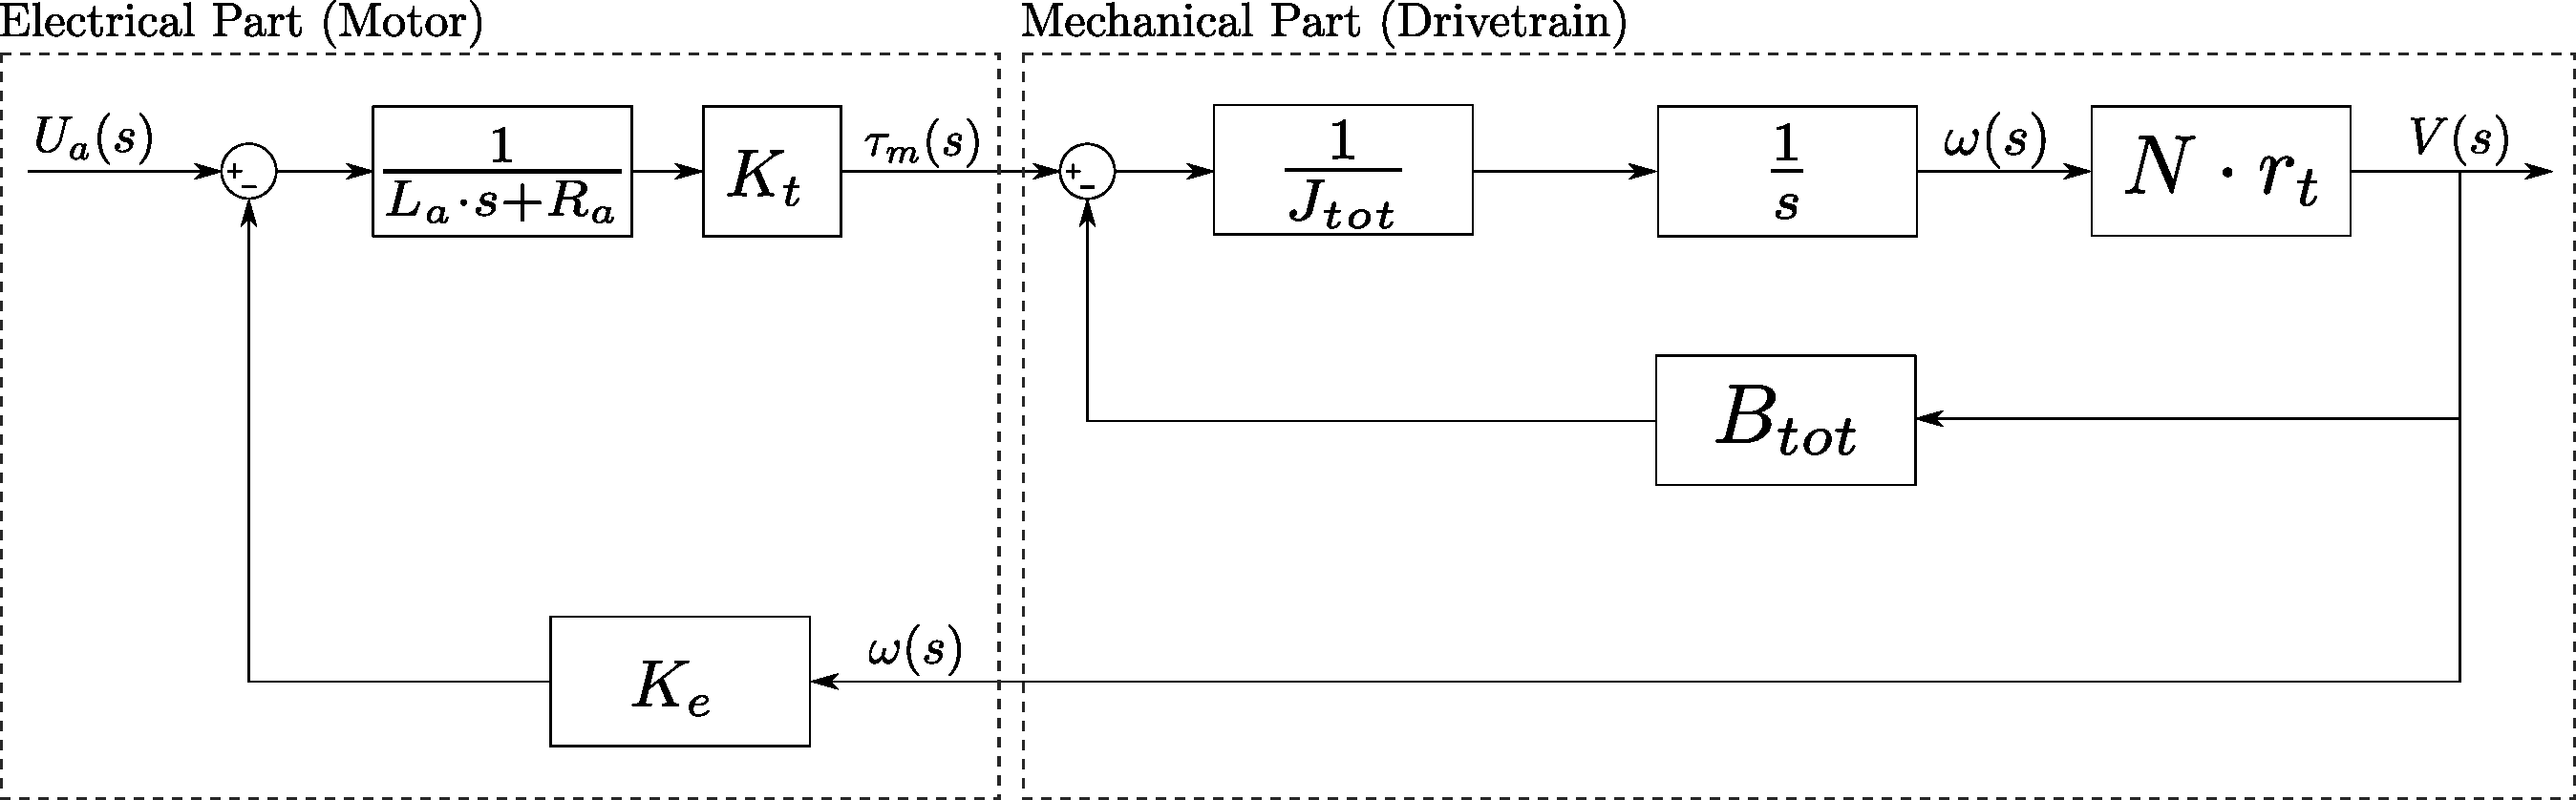
\includegraphics[width=\textwidth]{figures/totalVelocityModelDiagramNotComplicated.pdf}
	\caption{A block diagram of the combined drivetrain considering total inertia and friction acting on rotational velocity}
	\label{fig:BlockDiagramDrivetrainNotComplicated}
\end{figure}
%
In order to use this model in simulation, all terms must have a known value. To accomplish this, several tests has been carried out. The tests determining the generator constant, \si{K_e}, the motor constant, \si{K_t}, the armature inductance, \si{L_a}, and the armature resistance, \si{R_a}, are documented in \appref{app:motorTests}. The value of the total friction of the system, \si{B_{tot}}, is found in \appref{app:frictionTest} and the total inertia, \si{J_{tot}}, in \appref{app:inertiaTest}. The gear ratio, \si{N}, and the radius of the drive wheel, \si{r_t}, are measured directly on the vehicle.








